\documentclass[a4paper,10pt]{report}
\usepackage[utf8]{inputenc}
\usepackage{amssymb}
\usepackage{amsthm}
\usepackage{amsmath}
\usepackage{graphicx}

\setlength{\parindent}{0pt}

\begin{document}
\title{Modern Physics - Waves, Optics}
\author{Zack Garza}
\maketitle
\tableofcontents

\chapter{Geometric Optics}
\section{Reflection}
\begin{enumerate}
 \item Specular Reflection

 Reflection from a smooth surface that reflects rays parallel to each other. Occurs as long as the surface variations are much smaller than $\lambda$.

 \item Diffuse Reflection

 Reflection from a rough surface that reflects rays in various directions.

\end{enumerate}

In general, the angle of reflection will equal to angle of incidence, or
\begin{align*}
 \theta_{1}' &= \theta_1 \\
 (\text{Reflection Angle} &= \text{Incident Angle})
\end{align*}


\section{Refraction}
\subsection{Equations}

\begin{enumerate}
  \item
    Index of Refraction:
    \begin{align*}
        n &= \frac{c}{v_{\text{Medium}}} \text{ or } vn=c
    \end{align*}
    Defined as the ratio between the speed of light in a vaccum and in a medium. $v$ is always less than $c$, so $n>1$ for all substances.
    This also implies $\lambda_n < \lambda$, or that the wavelength of light in a medium is always lower than its wavelength in a vacuum.

  \item
    Snell's Law of Refraction:
    \begin{align*}
    n_1\sin\theta_1 &= n_2\sin\theta_2 \\
    \lambda_1 n_1 &= \lambda_2 n_2
    \end{align*}
    As light travels from one medium to another, its frequency does not change, but its wavelength \underline{does}.

  \item
    Total internal reflection:
    \begin{align*}
     &\sin\theta_{\text{crit}} = \frac{n_2}{n_1} &(\text{for } n_1 > n_2)
    \end{align*}
    Occurs when light travels from a medium with a high $n$ to one with a lower $n$, so $n_2/n_1 \le 1$.
    Can be in degrees or radians, just use the conversion
    \begin{align*}
     \frac{\text{radians}}{2\pi} = \frac{\text{degrees}}{360^{\circ}}
    \end{align*}
\end{enumerate}
\section{Homework Review}

\begin{figure}[h!]
  \begin{centering}
  \begin{center}
  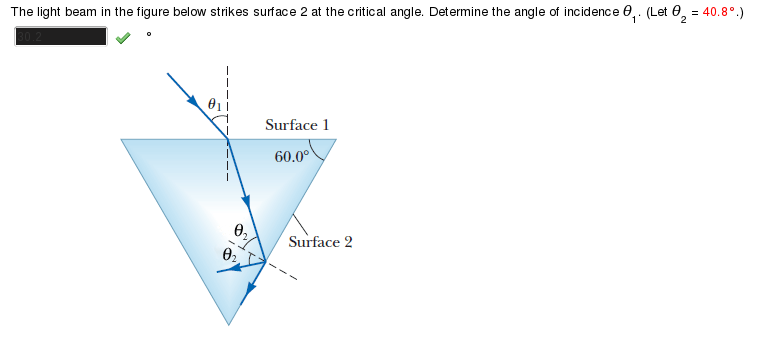
\includegraphics[width=\linewidth]{./prism.png}
  \caption{Determine angle of incidence, given the critical angle inside the prism.}
  \end{center}
  \par\end{centering}
  \end{figure}
  Hints: The sum of interior angles is always $180^{\circ}$. Solve for ratio of indices of refraction. Use Snell's Law.

  Solution: $30.2^{\circ}$.

\chapter{Image Formation: Mirrors, Lenses}

\section{Flat Mirrors}
  \begin{figure}[htpb]
  \begin{centering}
  \begin{center}
  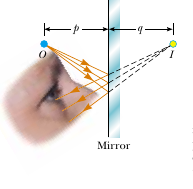
\includegraphics[]{./pqmirror.png}
  \label{fig:parallel_diagram}
  \caption{Conventions}
  \end{center}
  \par\end{centering}
  \end{figure}
  Conventions
  \begin{itemize}
   \item $O$: Object
   \item $I$: Image of object
   \item $p$: Actual distance of object
   \item $q$: Distance of Image
  \end{itemize}

\section{Conic Mirrors}
To determine image location, only three principle rays are essential:
\begin{enumerate}
 \item
    From the top of the object, parallel to the principal axis.

    (Reflected along line with $F$. Concave: Towards, Convex: Away)
 \item
    From the top of the object, through the focal point $f$.

    (Always reflected parallel to principal axis.)
 \item
    From the top of the object, through the center of curvature $C$.

    (Always reflected back upon itself)
\end{enumerate}
The intersection of these rays locates the image.

\subsection{Concave Mirrors}
The center of curvature $C$ is located on the principle axis. All paraxial rays (ones that diverge from the principle axis by only a small angle) converge on $I$, so objects placed farther away than $C$ (on the principle axis) produce a \textbf{real} image in front of the mirror. If rays emanating from $O$ instead tend to diverge from the principal axis, spherical aberration is introduced and the image becomes blurred.

Always has a \textbf{positive} focal length -- that is, $F$ is in front of the mirror.

If object is \textit{farther} than $C$, image is \textbf{real, inverted,} and \textbf{reduced} in size.

If the object is \textit{between} $C$ and the mirror, the image is \textbf{virtual, upright,} and \textbf{enlarged}.

\subsection{Convex Mirrors}
Always has \textbf{negative} focal length, where $F$ is located behind the mirror.
Images are always \textbf{virtual, upright,} and \textbf{reduced} in size.
\begin{figure}[h!]
  \begin{centering}
  \begin{center}
  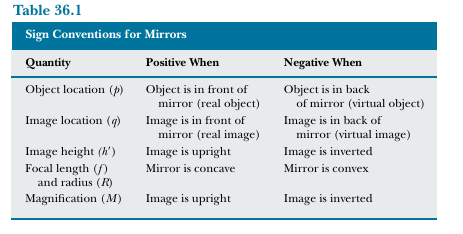
\includegraphics[width=\linewidth]{./mirrorsignconv.png}
  \label{fig:mirror_sign_conventions}
  \caption{Sign Conventions for Mirrors}
  \end{center}
  \par\end{centering}
  \end{figure}


\section{Equations}
\begin{enumerate}
  \item
  Definition of Magnification:
  \begin{align*}
   M = \frac{h'}{h}
  \end{align*}

  \item
  Magnification in a Concave Mirror:
  \begin{align*}
   M = \frac{-q}{p}
  \end{align*}
  $M<1$ indicates that the image is smaller than the object. $-M$ indicates image is inverted.

  \item
  The Mirror Equation:
  \begin{align*}
   \frac{1}{p} + \frac{1}{q} = \frac{1}{f} (\text{ where} f = \frac{R}{2})
  \end{align*}
  Depends only on the curvature of the mirror, and not its material.
  $+q$ denotes an image on the front side of the mirror (real), and vice-versa.

\section{Homework / Review}

\begin{figure}[h!]
  \begin{centering}
  \begin{center}
  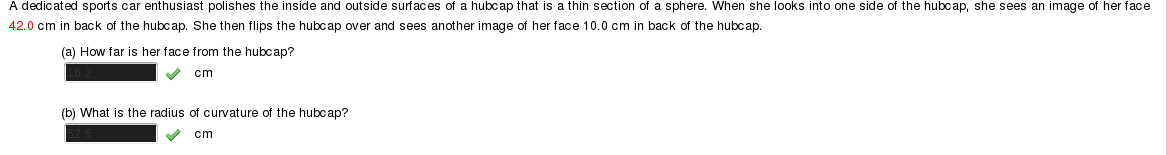
\includegraphics[width=\linewidth]{./hw5.png}
  \label{fig:hw_concave_convex}
  \caption{Convex/Concave Mirrors}
  \end{center}
  \par\end{centering}
  \end{figure}
  Hints: Results in two equations in two unknowns. Near image is convex, far image is concave. $F$ is negative for convex mirrors.

  Solutions: 16.2 cm, 52,5 cm.


\end{enumerate}


\end{document}
